\chapter{Introduction}

The fingerprint is the systematic compilation of a certain device in order to identify it, singularize it and profile it. This data set practically allows, univocally, to identify that device and the person or group of people who may be using it. In general, devices such as mobile phones, tablets, laptops and desktop computers are used by a single person and therefore, we can assume that the data collected from a certain device belongs to a specific person. \par

Currently, web applications provide services completely free of charge in exchange for the data they collect from users. In most cases, this information is profitable through marketing and advertising services that want to sell a specific product or service. Therefore, these services need to profile the user in order to offer them a product that may interest them. Entities use these data compilation mechanisms with all devices that connect to their servers, in order to monitor the user and create a profile. \par

The best-known tracking technique are cookies, which are stored on the device and then used to study the web application's usage and to improve the user experience. It is common to find privacy clauses that allow the user to consent or not to use them. Some browsers offer the possibility of disabling their use and some antivirus perform periodic deletions of the trace files, but most web applications do not allow access to their services if the user does not allow their cookies. The use of fingerprint techniques allows not lose the traceability of the user if cookies are deleted. Technologies such as JavaScript, Flash and Microsoft Silverlight, facilitate the implementation of methods to collect very specific information about the device, such as the screen size or the operating system version. The combination of these characteristics allows the user to be profiled and identified. \par

\section{Objetives}
 
El principal objetivo de este proyecto es crear una aplicación web que permita recopilar los datos de un terminal, aplicando las distintas técnicas de \textit{fingerprinting}, y elaborar un perfil en base a ellos. En concreto tenemos las siguientes metas:
\begin{itemize}
    \item Crear una aplicación escalable, para que en el futuro se pueda continuar desarrollando según se requiera.
    \item Investigar la variedad de métodos de huella digital e implementarlos.
    \item Almacenar la información recogida, de la cual se hará un perfilado y se guardará en una base de datos.
\end{itemize}

\section{Workplan}
Para el desarrollo del proyecto se ha fijado una planificación de tal forma que se cubre las fases de investigación, análisis de requisitos, implementación, testing y la memoria.\par
En la figura~\ref{fig:diagramaGantt} se puede observar el \textit{diagrama de Gantt}. Tras la ampliación de los plazos de entrega, se actualizaron las tareas posteriores y sus respectivos tiempos. Las tareas desglosadas consisten en:
\begin{itemize}
    \item \textbf{Investigación}: Recogida de información acerca de las distintas técnicas existentes\cite{Huella} para obtener información de los dispositivos. Esto incluye ciertas páginas que determinan la huella digital del navegador\cite{amiunique}.
    \item \textbf{Análisis de requisitos}: Valoración sobre qué lenguaje de programación y herramientas vamos a usar para el desarrollo del proyecto.
    \item \textbf{Implementación}: Puesta en marcha del proyecto. En esta etapa del desarrollo se implementaría la aplicación web con su respectiva base de datos.
    \item \textbf{Pruebas}: Comprobación del funcionamiento de la aplicación y resolución de las posibles incidencias.
    \item \textbf{Memoria}: Elaboración de la memoria.
\end{itemize}
\begin{figure}[b]
	%\centering
	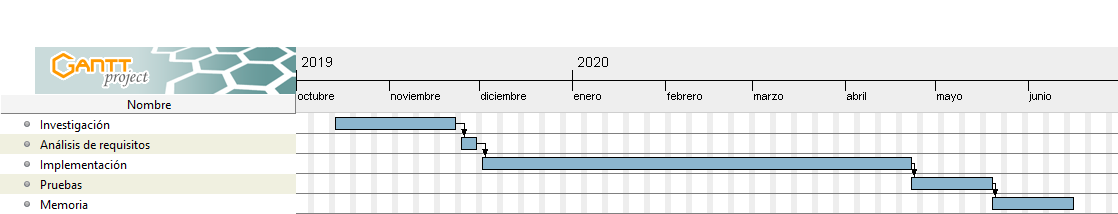
\includegraphics[width=1\textwidth, height=4cm]{Images/diagramaGantt.png}
	\caption{Gantt chart}
	\label{fig:diagramaGantt}
\end{figure}